\section{\large{Проектирование средства автоматизации}}
\addcontentsline{toc}{section}

\subsection{\Large{Стек технологий}}
\addcontentsline{toc}{subsection}

Во время проектирования системы всегда возникает ряд вопросов,
связанных с выбором стека технологий для решения следующих задач.

\begin{enumerate}
    \item Реализация программного кода
    \item Хранение данных
    \item Развертывание
    \item Тестирование
    \item Логирование
    \item Документация
    \item Протоколы взаимодействия
\end{enumerate}

Рассмотрим каждую из задач более подробно и выберем технологию, которая наиболее подходит для её решения в нашем случае.

\noindent \textbf{1. Язык программирования}.

В качестве основного языка программирования был выбран \textit{Python 3.8}\cite{PythonReference}.
Самым ценным ресурсом при реализации нашей системы является время разработки. Python является языком программирования
с динамической типизацией, имеет простой синтаксис,
а также очень большую базу готовых библиотек для решения любых задач.
Все эти преимущества позволяют, как быстро реализовывать функционал со стороны разработки, так и проводить проверку
разных алгоритмических гипотез за короткое время.

Такие недостатки Python, как низкая скорость выполнения программ и большое потребление памяти, в нашем случае
не играют решающей роли\cite{PythonProsAndCons}.
В Ubuntu 20.04 LTS -- операционной системе, на которой ведется разработка, установлен по умолчанию Python 3.8, поэтому
была выбрана именно эта версия языка.

\noindent \textbf{2. Хранение данных}.

Все данные, которые используются в проекте, достаточно однородны и могут быть легко представлены в табличном виде.
Поэтому в качестве технологии для хранения данных будем использовать реляционную базу данных.
Так как проектирование генеральных планов напрямую связано с геоданными, то необходимо учитывать это требование.

В качестве технического решения предлагается связка \textit{PostgreSQL 12} и расширения для работы с геоданными
\textit{PostGIS 3.1}. PostgreSQL является популярным open-source решением в мире баз данных,
а PostGIS содержит очень большое количество функций для преобразований геоданных, что нам очень важно\cite{PostGIS}.

\noindent \textbf{3. Развертывание}.

Необходимо предусмотреть механизм автоматического развертывания.
В компании используется система управления git-репозиториями \textit{GitLab}.
В этой системе доступен набор инструментов CI/CD, позволяющих решить данные задачи. Он называется \textit{GitLab-CI}
Так как разработка ведется на языке Python, то самым удобным способом развертывания приложений является технология 
Docker\cite{Docker}.

А для объединения нескольких \textit{Docker}-контейнеров вместе можно воспользоваться средствами \textit{docker-compose}.
Более сложные инструменты оркестрации контейнеров, такие как \textit{kubernetes} нам не требуются, в силу того, что у нас
только один вычислительный сервер.

\noindent \textbf{4. Тестирование}.

Наша система состоит из нескольких компонентов. Поэтому нужно предусмотреть следующие виды тестирования\cite{ArtOfTesting}.
\begin{itemize}
    \item \textit{Модульное тестирование}. Для проверки корректности работы различных функций и методов.
    \item \textit{Функциональное тестирование}. Для проверки соответствия результатов методов бизнес-требованиям.
    \item \textit{Интеграционное тестирование}. Для проверки, что все компоненты системы работают согласованно.
\end{itemize}

\noindent \textbf{5. Логирование}.

Помимо логирования в коде, требуется подумать о системе сбора, агрегации и хранения логов.
Одним из лучших решений на рынке является ELK. Это решение состоит из трех компонент: ElasticSearch для полнотекстового
поиска и аналитики, Logstash для сбора логов из приложений, Kibana для визуализации логов в веб-интерфейсе.

\noindent \textbf{6. Документация}.

Документацию имеет смысл писать только тогда, когда она действительно будет использоваться.
У нас таких случаев ровно два: документация API и документация математической библиотеки.

В первом случае, есть стандартные средства, как Swagger или GraphiQL,
которые позволяют генерировать документацию на основе модели данных автоматически.

Во втором случае требуется сгенерировать описание описание алгоритмов, используемых в программе.
Важная особенность в документировании алгоритмов заключается в том, что так как они зачастую очень сложны
в понимании только по текстовому описанию и требуют наличия иллюстраций. Это удобно делать в MarkDown- и LaTex-файлах.
Также нужно учесть, что в алгоритмах присутствует не только теоретическое обоснование, но и реализация, которая также
требует документации, но уже стандартными средствами разработки.

Чтобы объединить в себе два формата документации, теоретическую часть и реализацию,
воспользуемся инструментом Sphinx\cite{Sphinx}.

\noindent \textbf{7. Протоколы взаимодействия}.

В качестве основного протокола взаимодействия между сервисами будет использоваться
REST API over HTTP как легковесный и широко распространенный.
В качестве формата взаимодействия между веб-клиентом и сервером выберем формат JSON. Выберем его по следующим причинам:
\begin{itemize}
    \item Данный формат является человеко-читаемым и легко редактируется с помощью обычного текстового редактора,
    что в исследовательских задачах очень важно.
    \item В силу малого количества пользователей в системе, нам не требуется уделять особое внимание размеру
    передаваемых пакетов данных, что предоставляют бинарные форматы, такие как protobuf\cite{Protobuf}.
    \item Данный формат является очень популярным в индустрии и он имеет поддержку
    во всех современных языках программирования.
\end{itemize}


\noindent \textbf{Итого} при разработке системы будут использоваться следующий стек технологий:
\begin{itemize}
    \item Операционная система \textbf{Ubuntu 20.04 LTS}
    \item Язык программирования \textbf{Python 3.8.12}
    \item База данных \textbf{PostgreSQL 12} с расширением \textbf{PostGIS 3.1}
    \item Веб-сервер \textbf{nginx}
    \item Автоматическое развертывание \textbf{Gitlab-CI}
    \item Контейнеризация \textbf{Docker} и \textbf{docker-compose}
    \item Документация \textbf{OpenAPI} и \textbf{LaTex}
    \item Система сборки логов \textbf{ELK}
    \item Протоколы взаимодействия \textbf{REST API over HTTP}
\end{itemize}

\subsection{\Large{Системная архитектура}}
\addcontentsline{toc}{subsection}

\subsection{\Large{Пользователи системы и их потребности}}
\addcontentsline{toc}{subsection}

На текущий момент невозможно полноценно реализовать систему по автоматическому
формированию генеральных планов площадных объектов в силу отсутствия методики.
Для выработки этой методики требуется провести ряд исследований в области
алгоритмов формирования генпланов.

Любые исследования для реальных промышленных задач напрямую связаны с активной консультацией с техническими
экспертами со стороны заказчика, а также грамотного оформления всех результатов проведенных исследований
и быстрой возможностью их повторения.

На время научных изысканий система будет являться исследовательским прототипом.
Она должна позволять интерактивно отображать полученные результаты и фиксировать все проведенные эксперименты.

Можно выделить три группы пользователей, которые будут взаимодействовать с системой:
\begin{enumerate}
    \item {
        \textit{Технические эксперты со стороны заказчика.} Они обладают профессиональными знаниями в сфере
        проектирования генеральных планов площадных объектов. Именно на их экспертизе и базируется итоговое
        качество получаемого решения.
    }
    \item{
        \textit{Аналитики.} Они являются связкой между техническими экспертами и исследователями.
        Именно они презентуют полученные результаты техническим экспертам и подготавливают данные в том формате,
        которым могут воспользоваться исследователи.
    }
    \item{
        \textit{Исследователи.} Основной их деятельностью является решение именно математической задачи,
        применение и обоснование методики, которая будет давать наилучший результат.
    }
\end{enumerate}

С каждой из групп пользователей было проведено интервью с целью выяснения их потребностей в работе с системой
и был составлен список этих потребностей, который представлен ниже.

\begin{enumerate}
    \item {
        \textit{Технические эксперты со стороны заказчика}
        \begin{itemize}
            \item хотят иметь интерактивный доступ к результатам исследований на различных кейсах.
        \end{itemize}
    }
    \item {
        \textit{Аналитики}
        \begin{itemize}
            \item хотят иметь возможность загрузить данные, полученные от технических экспертов,
            \item хотят оперативно видеть результаты работы команды исследователей,
            \item хотят проводить анализ результатов различных методик, полученных на разных этапах развития проекта.
        \end{itemize}
    }
    \item {
        \textit{Исследователи}
        \begin{itemize}
            \item хотят иметь удобный и простой доступ к данным, полученные от технических экспертов,
            \item хотят иметь простой способ для отправки результатов новой методики для дальнейшего анализа команде аналитиков,
            \item хотят иметь возможность оперативно добавлять новые методики в действующий функционал системы.
        \end{itemize}
    }
\end{enumerate}

На основе потребностей пользователей можно составить несколько сценариев использования системы.
Для каждой группы пользователей эти сценарии будут несколько разными.
Ниже представлена диаграмма вариантов использования(см. рис\ \ref{pic:analysis__usecases-usecase}).

\begin{figure}[H]
	\hspace*{-2.5 cm}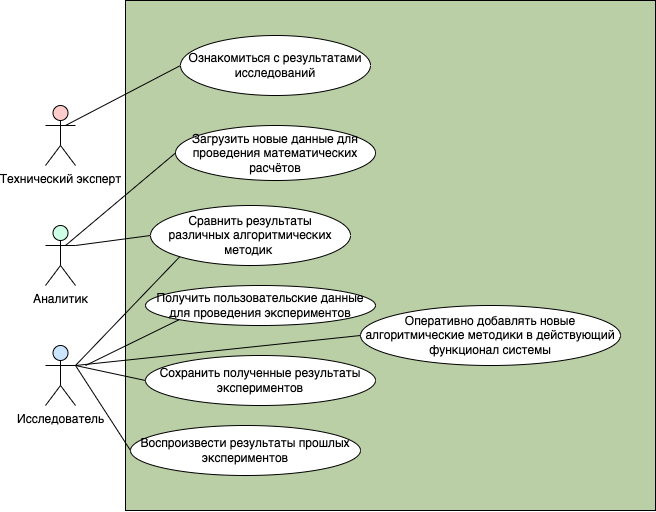
\includegraphics[width=0.6\textwidth, left]{analysis/pictures/usecases/usecase}
	\caption{Диаграмма вариантов использования}
	\label{pic:analysis__usecases-usecase}
\end{figure}
\vskip 5 mm


\subsection{\large{Сервис запуска математических методов}}
\addcontentsline{toc}{subsection}{\large{Сервис запуска математических методов}}

Детальная архитектура сервиса запуска математических методов представлена на диаграмме компонент
(см. рис\ \ref{pic:architecture__executor-component}).

\begin{figure}[H]
	\hspace*{-2.5 cm}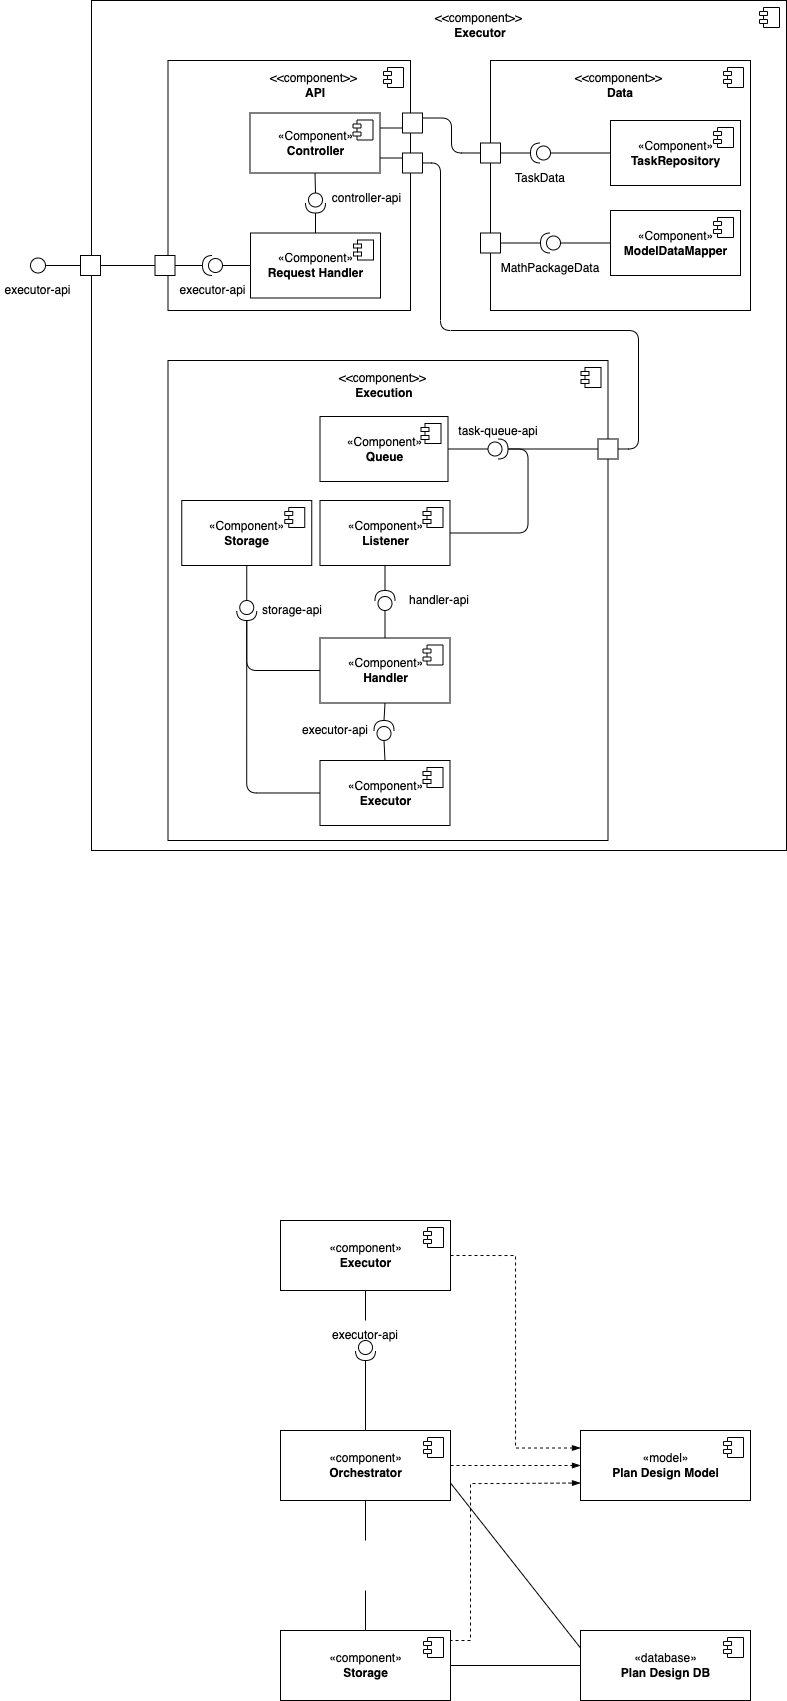
\includegraphics[width=\textwidth]{architecture/pictures/executor/component}
	\caption{Диаграмма компонент сервиса запуска математических методов}
	\label{pic:architecture__executor-component}
\end{figure}
\vskip 5 mm

Сервис представлен следующими компонентами:
\begin{enumerate}
	\item {
		\textbf{API} -- отвечает за предоставление REST API и отправки задачи в очередь.
		\begin{itemize}
			\item \textit{Request Handler}
			\item \textit{Controller}
		\end{itemize}
	}
	\item {
		\textbf{Data} -- отвечает за получение и сохранение данных.
		\begin{itemize}
			\item \textit{TaskRepository}
			\item \textit{ModelDataMapper}
		\end{itemize}
	}
	\item {
		\textbf{Execution} -- отвечает за запуск метода в отдельном процессе.
		\begin{itemize}
			\item \textit{Queue}
			\item \textit{Listener}
			\item \textit{Storage}
			\item \textit{Handler}
			\item \textit{Executor}
		\end{itemize}
	}
\end{enumerate}
\subsection{\large{Хранилище расчётных данных}}
\addcontentsline{toc}{subsection}{Хранилище расчётных данных}

Детальная архитектура хранилища расчётных данных представлена на диаграмме компонент
(см. рис\ \ref{pic:architecture__storage-component}).

\begin{figure}[H]
	\hspace*{-2.5 cm}\includegraphics[width=\textwidth]{architecture/pictures/storage/component}
	\caption{Диаграмма компонент хранилища расчётных данных}
	\label{pic:architecture__storage-component}
\end{figure}
\vskip 5 mm


Сервис представлен следующими компонентами:
\begin{enumerate}
	\item {
		\textbf{API} -- отвечает за предоставление REST API и отправки задачи в очередь.
		\begin{itemize}
			\item \textit{Request Handler}
			\item \textit{Controller}
		\end{itemize}
	}
	\item {
		\textbf{Repository} -- отвечает за получение и сохранение данных и логику их преобразований.
		\begin{itemize}
			\item \textit{ModelRepository}
			\item \textit{FeatureRepository}
			\item \textit{GlossaryRepository}
		\end{itemize}
	}
	\item {
		\textbf{Data} -- преобразование сущностей базы данных в сущности модели данных.
		\begin{itemize}
			\item \textit{FeatureMapper}
			\item \textit{GlossaryMapper}
		\end{itemize}
	}
	\item {
		\textbf{Database} -- связь с базой данных.
		\begin{itemize}
			\item \textit{Database} -- обеспечение CRUD-операций для сущностей базы данных.
		\end{itemize}
	}
\end{enumerate}
\subsection{\large{Cервис запуска расчётных задач}}
\addcontentsline{toc}{subsection}{Cервиc запуска расчётных задач}

Детальная архитектура сервиса запуска расчётных задач представлена на диаграмме компонент
(см. рис\ \ref{pic:architecture__orchestrator-component}).

\begin{figure}[H]
	\hspace*{-2.5 cm}\includegraphics[width=\textwidth]{architecture/pictures/orchestrator/component}
	\caption{Диаграмма компонент сервиса запуска расчётных задач}
	\label{pic:architecture__orchestrator-component}
\end{figure}
\vskip 5 mm

Сервис представлен следующими компонентами:
\begin{enumerate}
	\item {
		\textbf{API} -- отвечает за предоставление REST API и отправки задачи в очередь.
		\begin{itemize}
			\item \textit{Request Handler}
			\item \textit{Controller}
		\end{itemize}
	}
	\item {
		\textbf{Repository} -- отвечает за получение и сохранение данных и логику их преобразований.
		\begin{itemize}
			\item \textit{ModelRepository}
			\item \textit{FeatureRepository}
			\item \textit{GlossaryRepository}
		\end{itemize}
	}
	\item {
		\textbf{Data} -- преобразование сущностей базы данных в сущности модели данных.
		\begin{itemize}
			\item \textit{FeatureMapper}
			\item \textit{GlossaryMapper}
		\end{itemize}
	}
	\item {
		\textbf{Database} -- связь с базой данных.
		\begin{itemize}
			\item \textit{Database} -- обеспечение CRUD-операций для сущностей базы данных.
		\end{itemize}
	}
\end{enumerate}

%\subsection{\Large{Программная архитектура}}
%\addcontentsline{toc}{subsection}

%\subsection*{\large{Архитектура математической библиотеки}}
\addcontentsline{toc}{subsection}{Архитектура математической библиотеки}

Математическая библиотека занимает главенствующую роль в проекте, так как именно она содержит
набор алгоритмов, позволяющих получить генеральный план площадного объекта в автоматическом режиме.

Прежде чем изобразить архитектуру математической библиотеки, сформулируем основные концепции,
которые будут её описывать.
Для исследовательских проектов именно общие принципы реализации
приобретают главенствующую роль, так как в силу очень высокой динамичности обновления требований к системе
и несистемности этих требований отсутствует какая-либо возможность спроектировать архитектуру заранее.

\textit{Математическая методика} является классом алгоритмов, которые могут решать ту или иную задачу.
Каждая математическая методика используется хотя бы в одном \textit{математическом методе}.

\begin{itemize}
    \item {
        \textit{Аккуратное использование внешних зависимостей.}
        Исходный код математической библиотеки является главным результатом работы команды исследователей,
        поэтому, по-возможности, он должен содержать наименьшее количество внешних зависимостей.
        Допускается использование математических и научных библиотек языка Python.
    }
    \item {
        \textit{Каждая математическая методика должна быть выделена в отдельный программный модуль.}
        Так как каждая методика олицетворяет собой определенный класс математических алгоритмов,
        а сами алгоритмы являются концептуально сложными, то для упрощения их поддержки и модернизации
        следует ввести их явное логическое разделение.
    }
    \item {
        \textit{Минимализм во входных и выходных данных каждой методики.}
        В рамках каждой методики должны использоваться только лишь те данные, которые необходимы для её работы.
        Использования лишних данных следует избегать.
        Данная концепция обусловлена тем, что в силу высокой сложности алгоритмов,
        очень важно уменьшать накладные расходы на их отладку, что может сильно осложняться
        из-за большого количества входных параметров.
    }
    \item {
        \textit{Все параметры каждой методики должны быть выделены в отдельный класс.}
        Внутри реализации каждой математической методики недопустимо появление различных "магических чисел".
        Применение этой концепции обусловлено необходимостью повторяемости научного эксперимента.
        Если спрятать параметры алгоритма внутрь исходного кода, то результат на одних и тех же исходных данных
        может неудастся повторить в силу потерянного значения одного из чисел.
    }
    \item {
        \textit{Входные/выходные данные и параметры каждой методики должны быть сериализуемыми.}
        Так как расчёты могут производиться, как на сервере, так и на компьютере исследователя, то необходимо
        предусмотреть механизм простой передачи данных с компьютера на сервер и обратно. Самым простым способом
        является сериализация входных и выходных данных.
    }
\end{itemize}

Ниже представлена верхнеуровневая диаграмма классов модуля без конкретной реализации математических методов.

\begin{figure}[H]
	\hspace*{-2.5 cm}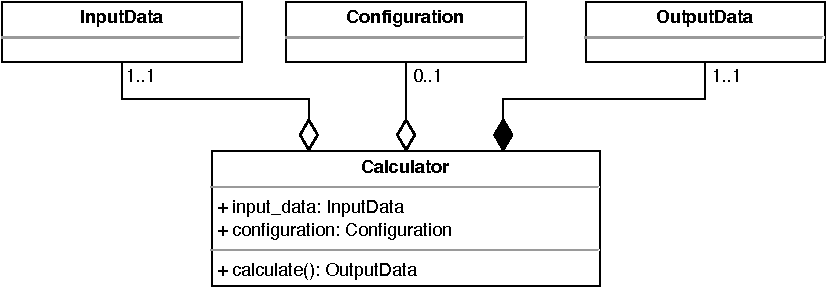
\includegraphics[width=0.6\textwidth, left]{architecture/pictures/math/classes}
	\caption{Верхнеуровневая диаграмма классов математического модуля}
	\label{pic:architecture__math-classes}
\end{figure}
\vskip 5 mm

%\subsection{\large{Разработка расчётной модели данных}}
\addcontentsline{toc}{subsection}

Расчётная модель данных состоит из расчётных элементов. Ниже представлена общая диаграмма классов расчётной модели данных
(см. рисунок \ref{pic:implementation__model-classes}).

\begin{figure}[H]
	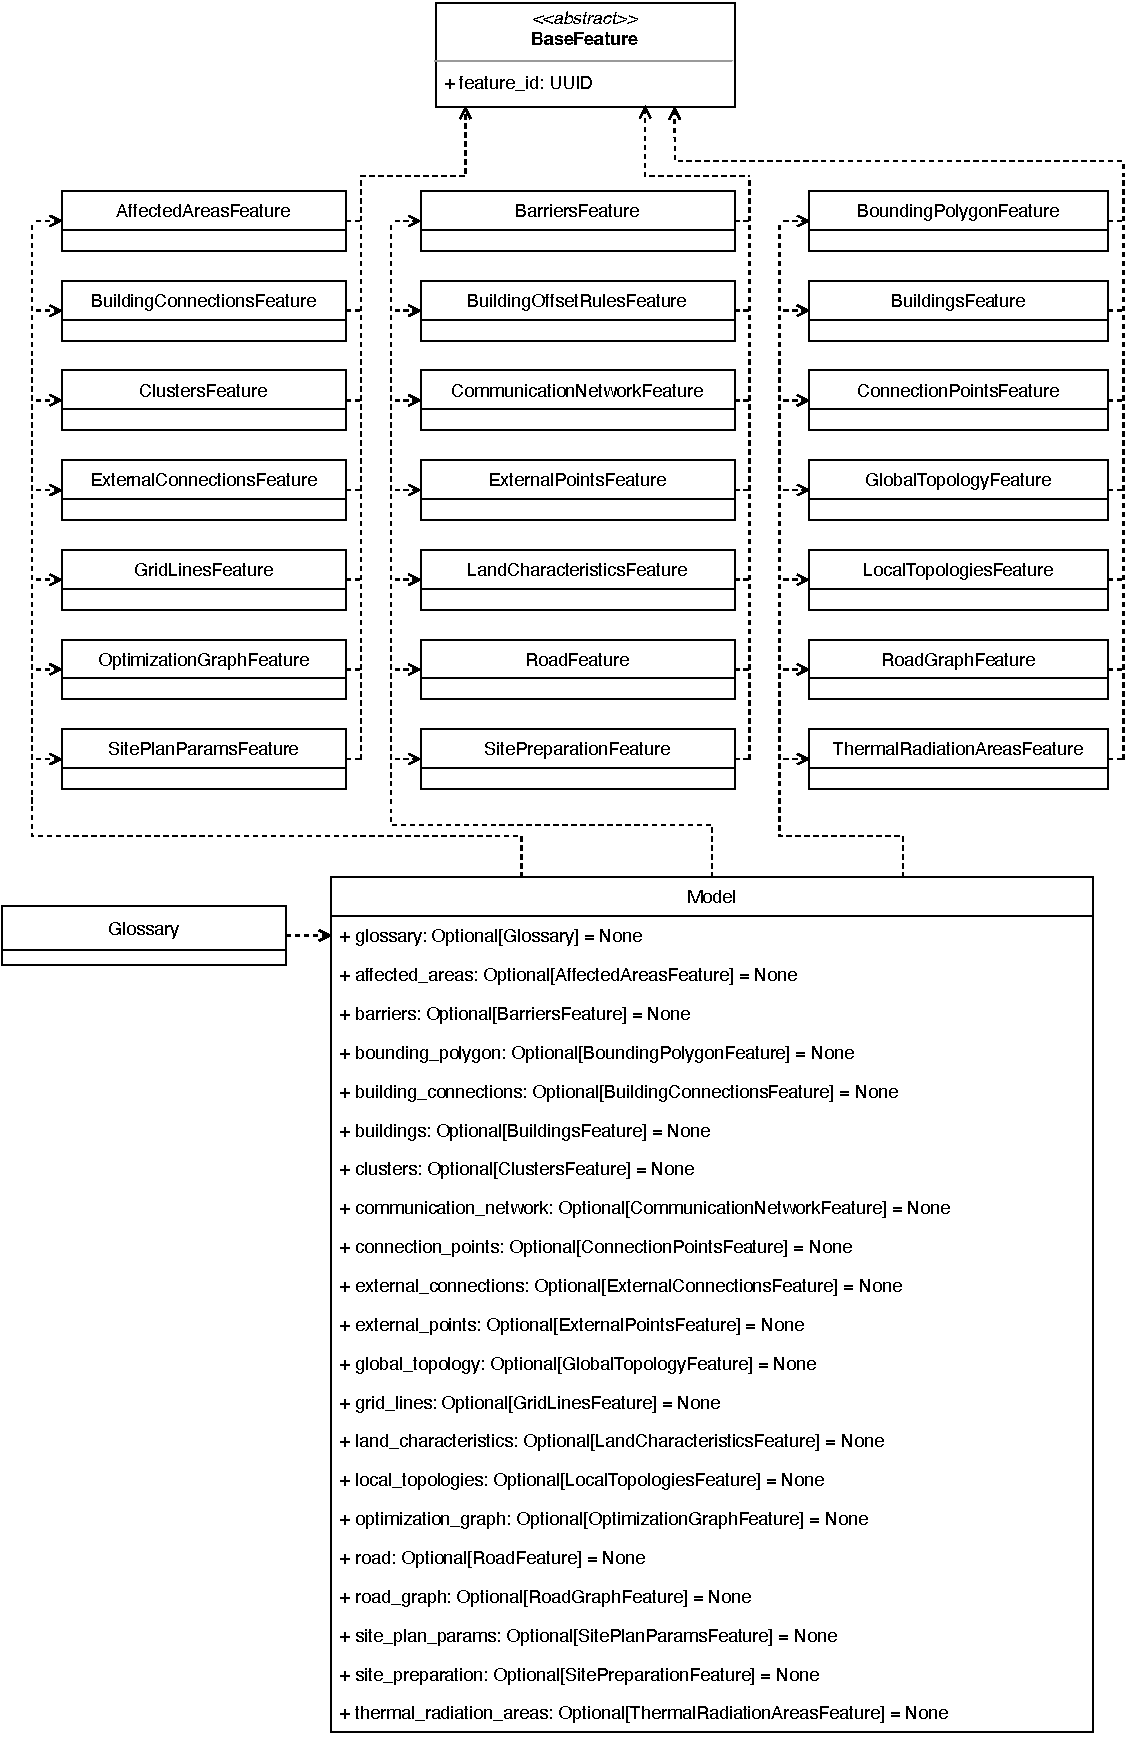
\includegraphics[width=0.8\textwidth]{implementation/pictures/model/classes}
	\caption{Общая диаграммма классов расчётной модели}
	\label{pic:implementation__model-classes}
\end{figure}
\vskip 5 mm

А вот диаграмма классов для расчётного элемента, описывающее сооружения(см. рисунок .\ref{pic:implementation__model-feature}).
\begin{figure}[H]
	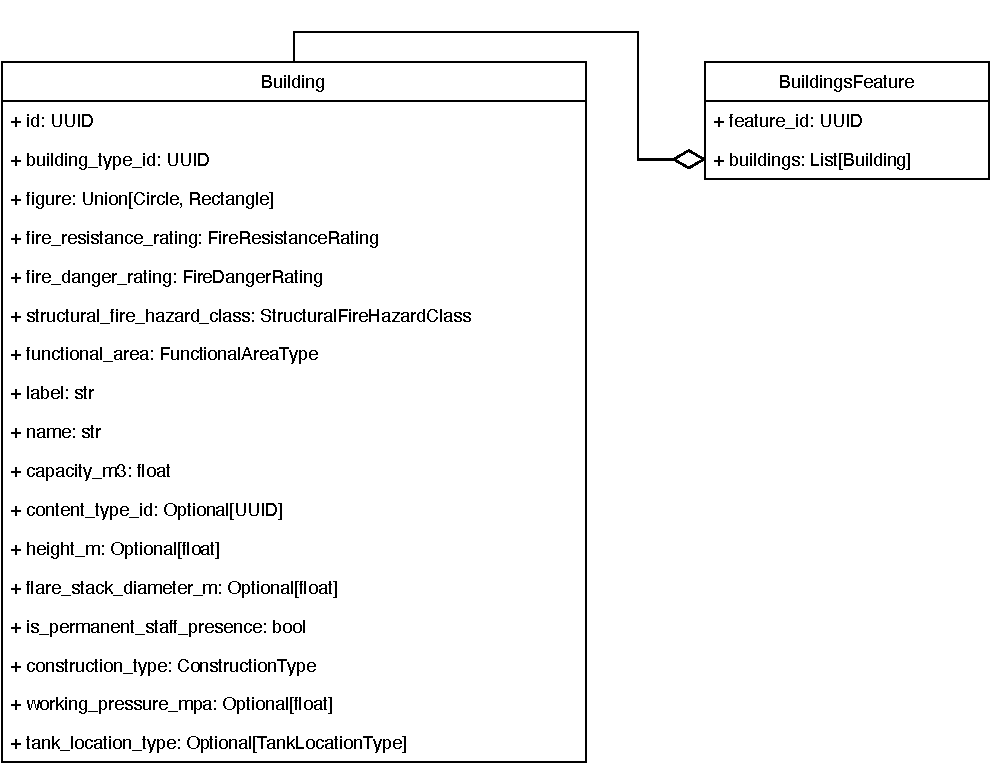
\includegraphics[width=0.8\textwidth]{implementation/pictures/model/feature}
	\caption{Общая диаграммма классов расчётной модели}
	\label{pic:implementation__model-feature}
\end{figure}


%\subsubsection{{Сервис запуска математических методов}}
\addcontentsline{toc}{subsubsection}

\begin{figure}[H]
	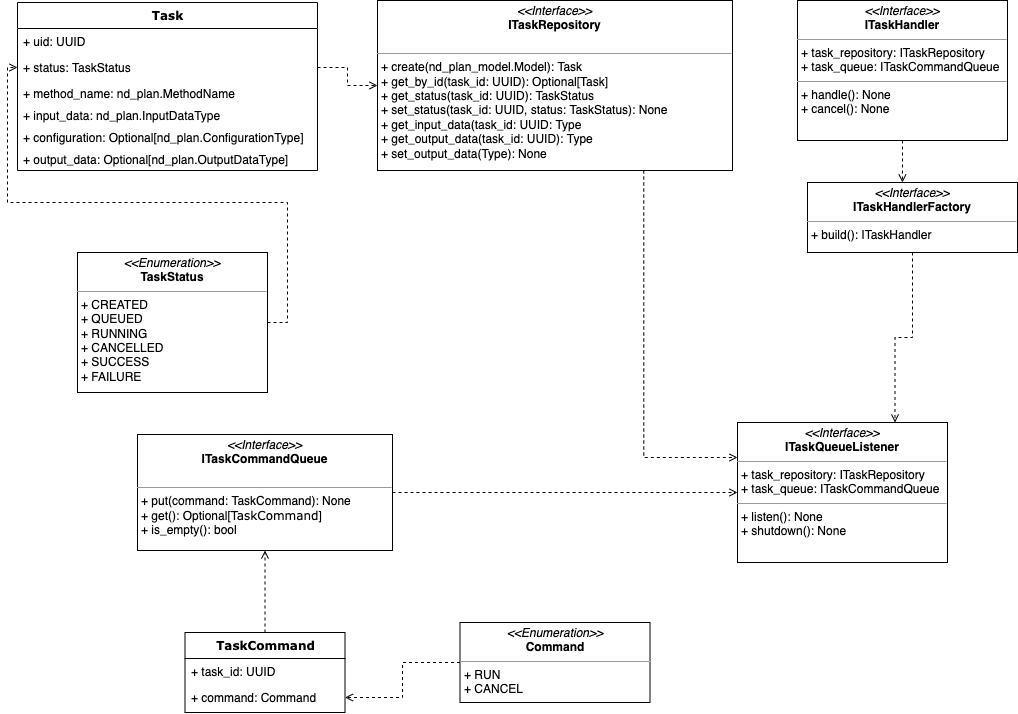
\includegraphics[width=\textwidth]{architecture/pictures/executor/execution_classes_diagram}
	\caption{Диаграмма классов расчетного модуля}
	\label{pic:architecture__execution-classes-diagram}
\end{figure}
\vskip 5 mm

Архитектура расчетного модуля представлена на диаграмме классов(см. рисунок \ \ref{pic:architecture__execution-classes-diagram}).
Основные классы и интерфейсы:
\begin{enumerate}
	\item \textit{Task} -- расчетная задача.
	\item \textit{TaskStatus} -- статус выполнения расчетной задачи.
	\item \textit{ITaskRepository} -- получения данных по расчётной задаче.
	\item \textit{ITaskHandler} -- запуск расчетных задач в отдельном процессе.
	\item \textit{ITaskCommandQueue} -- очередь задач.
	\item \textit{ITaskQueueListener} -- обработчик очереди задач, инициализация процесса расчета задач.
\end{enumerate}


\begin{figure}[H]
	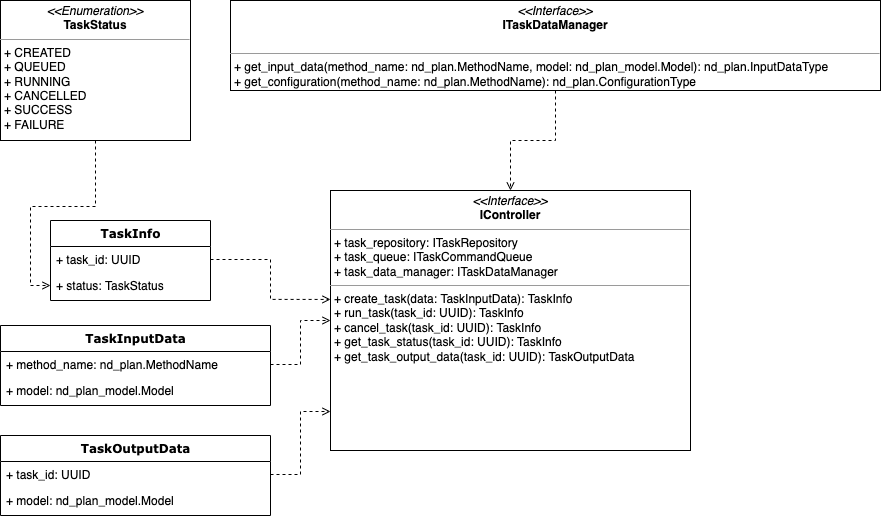
\includegraphics[width=\textwidth]{architecture/pictures/executor/api_classes_diagram}
	\caption{Диаграмма классов API}
	\label{pic:architecture__api-classes-diagram}
\end{figure}
\vskip 5 mm

Архитектура API представлена на диаграмме классов(см. рисунок \ \ref{pic:architecture__api-classes-diagram}).
Основные классы и интерфейсы:
\begin{enumerate}
	\item \textit{TaskInfo} -- информация о расчетной задаче.
	\item \textit{TaskStatus} -- статус выполнения расчетной задачи.
	\item \textit{TaskInputData} -- входные данные для создания расчетной задачи.
	\item \textit{TaskOutputData} -- результат расчета.
	\item \textit{ITaskDataManager} -- преобразование расчётной модели данных в модель данных математической библиотеки.
	\item \textit{IController} -- логика обработки запросов REST API.
\end{enumerate}
%\subsection{\large{Архитектура хранилища расчётных данных}}
\addcontentsline{toc}{subsection}


%\subsection*{\large{Архитектура сервиса запуска расчётных задач}}
\addcontentsline{toc}{subsection}{Архитектура сервиса запуска расчётных задач}

